%----------------------------------------------------------------------------------------
%	PACKAGES AND OTHER DOCUMENT CONFIGURATIONS
%----------------------------------------------------------------------------------------

\documentclass[12pt]{article}
\usepackage[spanish]{babel} %Tildes
\usepackage[extreme]{savetrees} %Espaciado e interlineado. Comentar si no gusta el interlineado.
\usepackage[utf8]{inputenc} %Encoding para tildes
\usepackage[breakable,skins]{tcolorbox} %Cajitas
\usepackage{fancyhdr} % Se necesita para el título arriba
\usepackage{lastpage} % Se necesita para poner el número de página
\usepackage{amsmath,amsfonts,amssymb,amsthm} %simbolos y demás
\usepackage{mathabx} %más símbolos
\usepackage{physics} %simbolos de derivadas, bra-ket.
\usepackage{multicol}
\usepackage[customcolors]{hf-tikz}
\usepackage[shortlabels]{enumitem}
\usepackage{tikz}
\usetikzlibrary{patterns}
\usepackage{siunitx}

%\def\darktheme
%%%%%%%%% === Document Configuration === %%%%%%%%%%%%%%

\pagestyle{fancy}
\setlength{\headheight}{14.49998pt} %NO MODIFICAR
\setlength{\footskip}{14.49998pt} %NO MODIFICAR

\ifx \darktheme\undefined

\lhead{Math161S2} % Nombre de autor
\chead{\textbf{Quiz 8 - Solutions}} % Titulo
\rhead{Name:\hspace*{5cm}}%\firstxmark} 
\lfoot{}%\lastxmark}
\cfoot{}
\rfoot{Page \thepage\ of\ \pageref{LastPage}} %A la derecha saldrá pág. 6 de 9. 
\else
\pagenumbering{gobble}
\pagecolor[rgb]{0,0,0}%{0.23,0.258,0.321}
\color[rgb]{1,1,1}
\fi

%%%%%%%%% === My T Color Box === %%%%%%%%%%%%%%

\ifx \darktheme\undefined
\newtcolorbox{ptcb}{
colframe = black,
colback = white,
breakable,
enhanced
}
\newtcolorbox{ptcbP}{
colframe = black,
colback = white,
coltitle = black,
colbacktitle = black!40,
title = Practice,
breakable,
enhanced
}

\else
\newtcolorbox{ptcb}{
colframe = white,
colback = black,
colupper = white,
breakable,
enhanced
}
\newtcolorbox{ptcbP}{
colframe = white,
colback = black,
colupper = white,
coltitle = white,
colbacktitle = black,
title = Practice,
breakable,
enhanced
}
\fi

%%%%%%%%% === Tikz para matrices === %%%%%%%%%%%%%%

\tikzset{
  style green/.style={
    set fill color=green!50!lime!60,
    set border color=white,
  },
  style cyan/.style={
    set fill color=cyan!90!blue!60,
    set border color=white,
  },
  style orange/.style={
    set fill color=orange!80!red!60,
    set border color=white,
  },
  row/.style={
    above left offset={-0.15,0.31},
    below right offset={0.15,-0.125},
    #1
  },
  col/.style={
    above left offset={-0.1,0.3},
    below right offset={0.15,-0.15},
    #1
  }
}

%%%%%%%%% === Theorems and suchlike === %%%%%%%%%%%%%%

\theoremstyle{plain}
\newtheorem{Th}{Theorem}  %%% Theorem 1.1
\newtheorem*{nTh}{Theorem}             %%% No-numbered Theorem
\newtheorem{Prop}[Th]{Proposition}     %%% Proposition 1.2
\newtheorem{Lem}[Th]{Lemma}             %%% Lemma 1.3
\newtheorem*{nLem}{Lemma}               %%% No-numbered Lemma
\newtheorem{Cor}[Th]{Corollary}        %%% Corollary 1.4
\newtheorem*{nCor}{Corollary}          %%% No-numbered Corollary

\theoremstyle{definition}
\newtheorem*{Def}{Definition}       %%% Definition 1.5
\newtheorem*{nonum-Def}{Definition}    %%% No number Definition
\newtheorem*{nEx}{Example}             %%% No number Example
\newtheorem{Ex}[Th]{Example}           %%% Example
\newtheorem{Ej}[Th]{Exercise}         %%% Exercise
\newtheorem*{nEj}{Exercise}           %%% No number Excercise
\newtheorem*{Not}{Notation}       %%% Definition 1.5

\theoremstyle{remark}
\newtheorem*{Rmk}{Remark}      %%%Remark 1.6

%\numberwithin{equation}{section}

\setlength{\parindent}{3ex}

%%====== Useful macros: =======%%%

\DeclareMathOperator{\gen}{gen}     %%%set generated by...
\DeclareMathOperator{\Rng}{Rng}     %%%rangomat
\DeclareMathOperator{\Nul}{Nul}     %%%rangomat
\DeclareMathOperator{\Proy}{Proy}   %%%proyección
\DeclareMathOperator{\id}{id}       %%%identity operator

\newcommand{\al}{\alpha}            %%%short for \alpha
\newcommand{\la}{\lambda}           %%%short for \lambda
\newcommand{\sg}{\sigma}            %%%short for \sigma
\newcommand{\te}{\theta}                %% short for  \theta
\renewcommand{\l}{\ell}

\newcommand{\thickhat}[1]{\mathbf{\hat{\text{$#1$}}}}
\newcommand{\ii}{\vu{\imath}}
\newcommand{\jj}{\vu{\jmath}}
\newcommand{\kk}{\thickhat{k}}

\newcommand{\bC}{\mathbb{C}}        %%%complex numbers
\newcommand{\bN}{\mathbb{N}}        %%%natural numbers
\newcommand{\bP}{\mathbb{P}}        %%%polynomials
\newcommand{\bR}{\mathbb{R}}        %%%real numbers
\newcommand{\bZ}{\mathbb{Z}}        %%%integer numbers
\newcommand{\cB}{\mathcal{B}}       %%%basis
\newcommand{\cC}{\mathcal{C}}       %%%basis
\newcommand{\cM}{\mathcal{M}}       %%%matrix family

\newcommand{\sT}{\mathsf{T}}        %%%traspuesta

\renewcommand{\geq}{\geqslant}      %%%(to save typing)
\renewcommand{\leq}{\leqslant}      %%%(to save typing)
\newcommand{\x}{\times}             %%%product
\renewcommand{\:}{\colon}           %%%colon in  f: A -> B
\newcommand{\isom}{\simeq}              %% isomorfismo

\newcommand{\un}[1]{\underline{#1}}
\newcommand{\half}{\frac12}

\newcommand*{\Cdot}{{\raisebox{-0.25ex}{\scalebox{1.5}{$\cdot$}}}}      %% cdot más grande
\renewcommand{\.}{\Cdot}                %% producto escalar

\newcommand{\twobyone}[2]{\begin{pmatrix} %% 2 x 1 matrix
  #1 \\ #2 \end{pmatrix}}
  \newcommand{\twobytwo}[4]{\begin{pmatrix} %% 2 x 2 matrix
    #1 & #2 \\ #3 & #4 \end{pmatrix}}
    \newcommand{\twobythree}[6]{\begin{pmatrix} %% 2 x 3 matrix
        #1 & #2 & #3\\ #4 & #5 & #6 \end{pmatrix}}
\newcommand{\threebyone}[3]{\begin{pmatrix} %% 3 x 1 matrix
  #1 \\ #2 \\ #3 \end{pmatrix}}
  \newcommand{\threebytwo}[6]{\begin{pmatrix} %% 3 x 1 matrix
    #1 & #2\\ #3 & #4\\ #5&#6 \end{pmatrix}}
\newcommand{\threebythree}[9]{\begin{pmatrix} %% 3 x 3 matrix
  #1 & #2 & #3 \\ #4 & #5 & #6 \\ #7 & #8 & #9 \end{pmatrix}}

\newcommand{\To}{\Rightarrow}

\newcommand{\vaf}{\overrightarrow}

\newcommand{\set}[1]{\{\,#1\,\}}    %% set notation
\newcommand{\Set}[1]{\biggl\{\,#1\,\biggr\}} %% set notation (large)
\newcommand{\red}[1]{\textcolor{red}{#1}}
\newcommand{\blu}[1]{\textcolor{blue}{#1}}

%----------------------------------------------------------------------------------------
%	ARTICLE CONTENTS
%----------------------------------------------------------------------------------------

\begin{document}
%\begin{multicols}{2}

\begin{Ej}
 Consider the series $\displaystyle\sum_{n=1}^{\infty}\frac{3\sqrt{n^3}}{7n^{5r}}$ where $r$ is a real number and do the following:
 \begin{enumerate}[i)]
  \itemsep=-0.4em
  \item Identify the general term of the series and simplify it.
  \item Is our series a $p$-series? How can you justify that?
  \item State the convergence result for $p$ series. This means, given ANY $p$-series $\sum \frac{1}{n^p}$, for what values of $p$ will that converge?
  \item Determine for which values of $r$ will our series converge. [Hint: The answer to this item is NOT the same as the last item.]
 \end{enumerate}
\end{Ej}

\begin{ptcb}
\begin{enumerate}
  \itemsep=-0.4em
  \item The general term is $\frac{3\sqrt{n^3}}{7n^{5p}}$. We may simplify it to $\frac{3}{7}\frac{1}{n^{5r-3/2}}$.
  \item Indeed it's a $p$-series, as the general term looks like $1$ over $n$ to some power, in this case $5r-\frac32$.
  \item A general $p$ series converges when $p>1$. 
  \item We require that $5r-\frac{3}{2}>1$ so solving for $r$ we get $5r>\frac{5}{2}$ which means that $r>\frac{1}{2}$. So for values of $r$ larger than $\frac12$, our series converges.
\end{enumerate}
\end{ptcb}

\begin{Ej}[Filling a triangle]
  Consider an empty triangle of area $A$ which we start filling with smaller triangles. The objective of this question is to determine if we can fill completely the triangle in question.\par 
  \begin{figure*}[h]
    \centering
    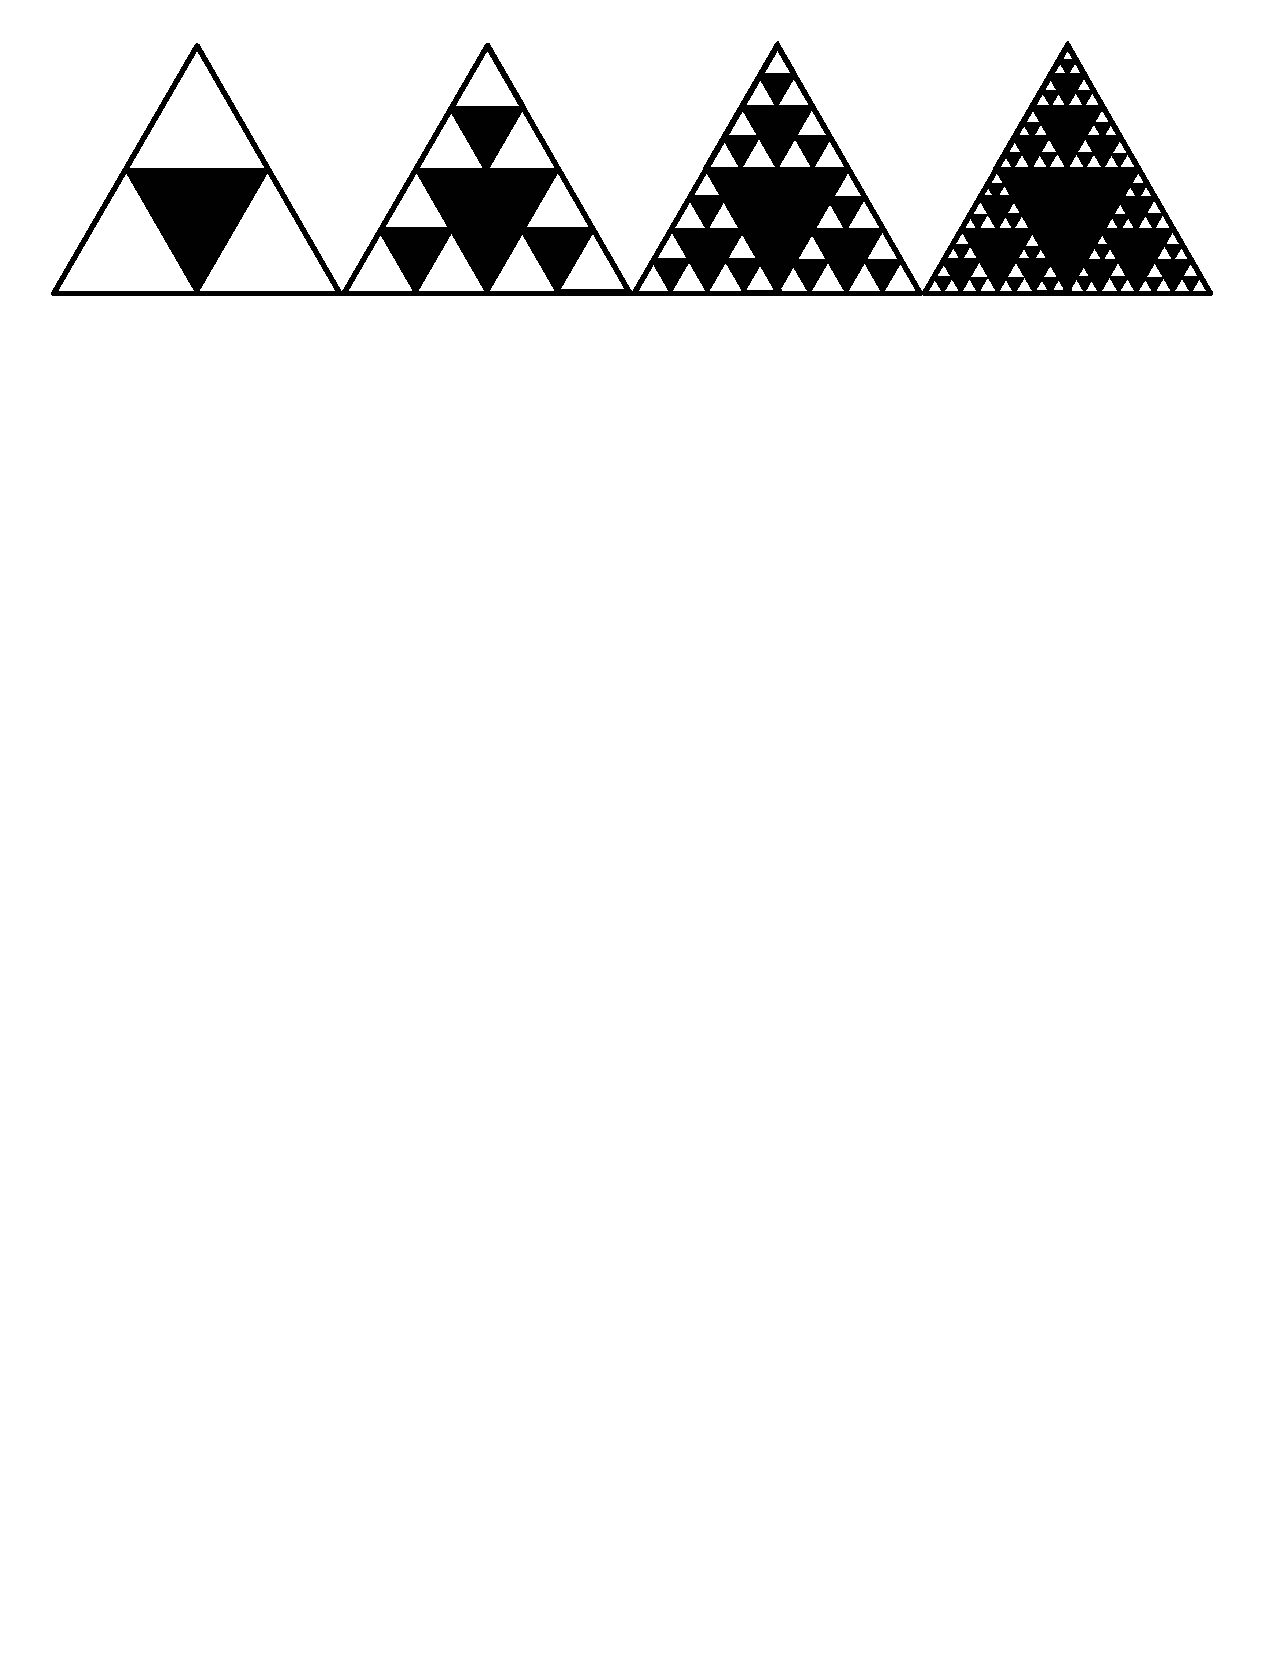
\includegraphics[width=0.8\textwidth, trim= 0.92cm 23.2cm 1.05cm 0.5cm,clip]{fig1.pdf}
  \end{figure*}
  We start adding a triangle with area $a_1=\frac{A}{4}$ in the middle, then the second step adds $3$ triangles of area $\left(\frac{A/4}{4}\right)=\frac{A}{16}$. So in total we are adding an area of $a_2=\frac{3A}{16}$.
 \begin{enumerate}[i)]
  \itemsep=-0.4em
  \item In the third step, how many triangles do we add? What is the area of each of the new smaller triangles? In total how much area $a_3$ are we adding in the third step?
  \item Derive a formula for the area added $a_n$ at the $n^{\text{th}}$ step by considering how many triangles are we adding and the area of each of those new triangles.
  \item As a sequence, is $a_n$ geometric? If it is, what's is initial term and common ratio?
  \item Consider the series $\sum_{n=1}^{\infty}a_n$, in terms of area, what does this series represent? What do the partial sums represent?
  \item Using the information above, determine if we fill up the triangle.
 \end{enumerate}
\end{Ej}

\begin{ptcb}
  \begin{enumerate}
    \itemsep=-0.4em
    \item TO DO
  \end{enumerate}
  \end{ptcb}

%\end{multicols}
\end{document} 